\chapter{Konzeption}

Nisi et sed provident esse accusamus consequuntur praesentium qui. Eaque vel non dolores aliquam fuga voluptas quia sit. Vel ut rem et in quis quo inventore quidem. Enim quam voluptatum atque et. Consequuntur repellendus quia voluptate vel quia et suscipit soluta. Fugiat iste corporis voluptatem molestiae.

\section{Funktionalität} \label{sec:concept-func}

Im Folgenden werden die zuvor konzipierten Funktionalitäten des Systems
vorgestellt, welche die zuvor festgelegten Anforderungen (s.
\autoref{sec:analysis-anf}) erfüllen sollen. Zuerst werden die übernommenen und
überarbeiteten Funktionalitäten der EMI-Award-App dargelegt. Anschließend werden
neue Funktionalitäten vorgestellt.

\subsection{Übernommene \& angepasste Funktionalitäten}

Die Funktionalitäten der EMI-Award-App (s. \autoref{table:emi-func}) dienen für
diese Arbeit als Grundlage. Um die Systemarchitektur später einfacher abbilden
zu können, werden die Funktionalitäten nach Nutzungsgruppe gruppiert (s.
\autoref{table:funk-old}). Aufgrund der abweichenden Anforderungen zur
EMI-Award-App müssen einige Funktionalitäten angepasst werden. Im Folgenden
werden die übernommenen und überarbeiteten Funktionalitäten für Veranstaltende
und Teilnehmende präsentiert.

\begin{table}[htpb]
    \def\arraystretch{1.25}
    \centering
    \caption{Übernommene Funktionalitäten der EMI-Award-App}
    \label{table:funk-old}
    \begin{tabular}{lll}
        \uzlhline%
        \uzlemph{ID} & \uzlemph{Titel}                            & \uzlemph{Anforderungen} \\
        \uzlhline%
        Ft-V-1       & Eintragen und Verwalten von Stationen      & \anfref{F11}            \\
        Ft-V-2       & Eintragen und Verwalten von Abzeichen      & \anfref{F12}            \\
        Ft-V-3       & Eintragen und Verwalten von Hilfseinträgen & \anfref{F13}            \\
        Ft-V-4       & Eintragen und Verwalten der Einführung     & \anfref{F14}            \\
        Ft-T-1       & Interaktive Karte mit Stationen            & \anfref{F30}            \\
        Ft-T-2       & Auflistung der Stationen                   & \anfref{F30}            \\
        Ft-T-3       & Virtuelles Besuchen mit QR-Code            &                         \\
        Ft-T-4       & Abzeichen                                  & \anfref{F60}            \\
        Ft-T-5       & Bedienungshilfe                            & \anfref{F50}            \\
        Ft-T-6       & Einleitende Slideshow                      & \anfref{F40}            \\
        \uzlhline
    \end{tabular}
\end{table}

Für die Veranstaltenden wurden einige Anpassungen vorgenommen. Das Eintragen der
Stationen (Ft-V-1), Abzeichen (Ft-V-2), Hilfseinträge (Ft-V-3) und Einführung
(Ft-V-4) muss an die Verallgemeinerung des Frameworks angepasst werden. Da der
Kontext der EMI-Award-App sehr spezifisch ist, waren die Anpassungsmöglichkeiten
auf das nötige beschränkt. Konkret wurden einige Daten in der App fest
eingebaut. Dies umschließt die Icons von Stationen und Abzeichen, die
Abschlussbedingung der einzelnen Abzeichen, sowie die Bilder der Einführung. All
diese Einstellungen sind nun frei anpassbar. Zudem werden mediale Inhalte für
Stationen nun nicht mehr benötigt, da diese nicht für jede Veranstaltung von
Bedeutung sind. Icons hingegen müssen für Stationen angegeben werden.\\
Zusätzlich werden zudem zwei neue Abschlussbedingungen eingeführt: eine
Textabgabe und eine Bildabgabe, welche von Veranstaltenden manuell akzeptiert
oder abgelehnt werden können.

Die Hilfseinträge (Ft-V-3) werden weitergehend überarbeitet, um eine größere
Anzahl an Einträgen übersichtlich anzuzeigen. Hierzu werden die Einträge
nach Kategorie gruppiert und in einem „Frage \& Antwort“ (FAQ) Format angegeben.
Somit wäre eine mögliche Frage „Wann endet die Veranstaltung?“, eingeordnet in
der Kategorie „Organisatorisches“.
% TODO: Markdown wichtig?

Eine weitere Überarbeitung betrifft das Eintragen und Verwalten der Einführung
(Ft-V-4), welche nun weitere Folienformate unterstützt. Das Layout der
EMI-Award-App hat ein festgesetztes Bild mit anpassbarem Text darunter
angezeigt. Stattdessen werden drei neue Formate eingeführt: Titelfolie (Bild +
Text), Bildfolie (Text + Bild) und eine ausschließliche Textfolie.

\subsection{Neue Funktionalitäten}

Um alle aufgestellten Anforderungen abzudecken, wurden zudem einige neue
Funktionalitäten konzipiert. Diese werden in \autoref{table:funk-new}
präsentiert und im Folgenden näher ausgeführt.

\begin{table}[htpb]
    \def\arraystretch{1.25}
    \centering
    \caption{Neue Funktionalitäten}
    \label{table:funk-new}
    \begin{tabular}{lll}
        \uzlhline%
        \uzlemph{ID} & \uzlemph{Titel}                    & \uzlemph{Anforderungen}   \\
        \uzlhline%
        Ft-V-5       & Benachrichtigungen an Teilnehmende & \anfref{F70}              \\
        Ft-V-6       & Feedbackanfragen                   & \anfref{F80}              \\
        Ft-V-7       & Statistiken zur Veranstaltung      & \anfref{F20}              \\
        Ft-V-8       & Zentrales Dashboard zur Verwaltung & \anfref{F10}~\anfref{F90} \\
        Ft-T-7       & Gruppen                            & \anfref{F100}             \\
        Ft-T-8       & Manuelle Abzeichen                 & \anfref{F60}              \\
        \uzlhline
    \end{tabular}
\end{table}


Die Benachrichtigungen in \textit{Ft-V-5} können von Veranstaltenden über das
Dashboard in \textit{Ft-V-8} an Teilnehmende gesendet werden. Die
Benachrichtigungen bestehen dabei aus Titel und einem Textinhalt. Alle bereits
gesendeten Benachrichtigungen können in einer Tabelle eingesehen werden. Die
Teilnehmenden erhalten beim Senden einer Benachrichtigung in der Web-App eine
Push-Benachrichtigung, welche die Eingaben der Veranstaltenden beinhaltet.
Sollten Teilnehmende zum Zeitpunkt des Absendens der Benachrichtigung die
Web-App nicht offen haben, so wird die Benachrichtigung zum nächsten Öffnen der
App präsentiert.

Die Feedbackanfragen aus \textit{Ft-V-6} geschehen in ähnlicher Form wie
\textit{Ft-V-5}. Erneut können Veranstaltende über das Dashboard aus
\textit{Ft-V-8} anfragen abschicken, welche Teilnehmende mit einem
Feedbackdialog präsentiert. Im Gegensatz zur Benachrichtigung können
Veranstaltende bei einer Feedbackanfrage einen Titel und auswählbare Gründe für
ein schlechtes Feedback angeben, um jedem Veranstaltungstypen gerecht zu werden.
Teilnehmende können aus drei möglichen Bewertungen wählen: „Gut“, „Mittelmäßig“
und „Schlecht“, welche als Emojis präsentiert werden. Bei einer Wahl von
„Mittelmäßig“ oder „Schlecht“ können Teilnehmende anschließend aus den, von
Veranstaltenden angegeben, Gründen auswählen und alternativ einen eigenen Grund
angeben. Das abgesendete Feedback wird Veranstaltenden anschließend im Dashboard
präsentiert.

Zusätzlich werden auch die Statistiken aus \textit{Ft-V-7} im
Dashboard aus \textit{Ft-V-8} angezeigt. Diese werden unterteilt in „Stationen“,
„Abzeichen“, „Teilnehmende“ und „Feedback“. Zu Stationen, Abzeichen und
Teilnehmenden werden die kumulativen, täglichen und durchschnittlichen täglichen
Besuche, neue Teilnehmende und Abzeichenabschlüsse angezeigt. Für Stationen und
Abzeichen werden zusätzlich die kumulativen Besuche und Abschlüsse pro Station
und Abzeichen angezeigt. Die kumulativen und täglichen Daten werden in Form
eines Graphen angezeigt. \\
In der Kategorie Feedback werden die insgesamt eingetroffenen Antworten, ihre
Bewertungen und die drei häufigsten angegebenen Gründe für schlechte Bewertungen
angezeigt. Zudem werden alle Antworten individuell in einer Tabelle dargestellt,
in der auch die eigenen Gründe der Teilnehmenden vorhanden sind.

Das Dashboard aus \textit{Ft-V-8} beinhaltet, neben den bereits erläuterten
Funktionen, eine Ansicht zur Bearbeitung der eingereichten Text- und
Bildabzeichen, sowie Eintragung und Verwaltung der Rahmendaten. Alle offenen
Einreichungen für Abzeichen, welche eine manuelle Bearbeitung bedürfen, werden
in einer Liste angezeigt und können ausgewählt werden, um die Einreichung zu
betrachten und zu bewerten. Die Rahmendaten der Veranstaltung lassen sich
separat davon verwalten. Sie umfassen Titel, Logo, Anfang und Ende der
Veranstaltung, sowie optionale Funktionen, ein Link zu weiteren Informationen
der Veranstaltung, das initiale Zentrum der interaktiven Karte und rechtliche
Informationen wie Impressum und Datenschutzerklärung.

Des Weiteren haben Teilnehmende die Möglichkeit Aktivitäten als Gruppen
(\textit{Ft-T-7}) abzuschließen. Hierzu gehört das Besuchen von Stationen und
das Abschließen von Abzeichen. Beim ersten Aufruf wird Teilnehmenden die
Möglichkeit gegeben eine Gruppe zu erstellen oder einer Gruppe beizutreten. Dies
geschieht über das Scannen des QR-Codes eines Gruppenmitglieds oder alternativ
mit der manuellen Eingabe des Gruppen-Codes. Zudem können Teilnehmende die
Gruppe jederzeit verlassen, eine neue erstellen oder einer anderen Beitreten.
Die Gruppen-Funktion kann von Veranstaltenden im Dashboard aus \textit{Ft-V-8}
eingestellt werden. Gruppen können erforderlich, optional oder ausgeschaltet
sein.

Abschließend stellen manuelle Abzeichen aus \textit{Ft-T-8} die letzte neue
Funktionalität dar, welche die manuelle Bearbeitung durch Veranstaltende
benötigen. Dazu gehören Text- und Bildabzeichen, sowie das manuelle Bestätigen
eines Abzeichens. Durch sie erhalten Teilnehmende die Möglichkeit kleine Texte
oder Bilder bei entsprechenden Abzeichen abzugeben. Nach der Abgabe können
Veranstaltende, wie in der Dashboard-Funktionalität beschrieben, die Einreichung
akzeptieren oder ablehnen. Sollte die Einreichung abgelehnt werden, können
Teilnehmende erneut eine Abgabe einreichen. Andernfalls wird das Abzeichen als
abgeschlossen markiert. \\
Insgesamt gibt es somit nun folgende Abschlussbedingungen: \textit{Anzahl
    besuchter Stationen}, \textit{Abschließen aller (anderen) Abzeichen},
\textit{Textabgabe}, \textit{Bildabgabe} und \textit{Manuelles akzeptieren}

\section{Interface-Design}

In diesem Abschnitt wird die Benutzeroberfläche aus Sicht der Veranstaltenden
und Teilnehmenden vorgestellt.

\subsection{Veranstaltende}



\subsection{Teilnehmende}

Die Grundlage der Benutzeroberfläche der Teilnehmenden bildet der Entwurf der
EMI-Award-App, welcher im Rahmen des dazugehörigen Bachelorprojekts bereits
evaluiert wurde. Es wurden einige Anpassungen vorgenommen, um die Usability
Heuristiken nach \textcite{Nielsen1994} zu beachten (\anfref{Q40}). Diese werden im Verlauf mit
ihren IDs referenziert (s. \autoref{table:nielsen}).

\begin{table}[htpb]
    \def\arraystretch{1.25}
    \centering
    \caption{Die Zehn Usability Heuristiken \cite{Nielsen1994}}
    \label{table:nielsen}
    \begin{tabular}{ll}
        \uzlhline%
        \uzlemph{ID} & \uzlemph{Heuristik}                         \\
        \uzlhline%
        H1           & Sichtbarkeit des Systemstatus               \\
        H2           & Übereinstimmung von System und Wirklichkeit \\
        H4           & Beständigkeit und Standards                 \\
        H6           & Wiedererkennung statt Erinnerung            \\
        H7           & Flexibilität und Effizienz                  \\
        H8           & Ästhetisches und minimalistisches Design    \\
        H10          & Hilfe und Dokumentation                     \\
        \uzlhline
    \end{tabular}
\end{table}

Da auf dem Entwurf der EMI-Award-App aufgebaut wird, wurde direkt mit einem
High-Fidelity Prototypen begonnen. Dieser wurde mit dem Interface-Design-Tool
Figma erstellt. Das Design der EMI-Award-App ist spezifisch auf die dazugehörige
Veranstaltung abgestimmt. Um eine möglichst neutrale und anpassbare Darstellung
zu ermöglichen (\anfref{F130}), wurde das Design dies hingehend angepasst.
Konkret wurden bewusst auf Farben verzichtet und EMI-Award spezifische Grafiken
entfernt oder durch Platzhalter ersetzt.

\begin{figure}[htpb]
    \begin{minipage}{.33\textwidth}
        \centering
        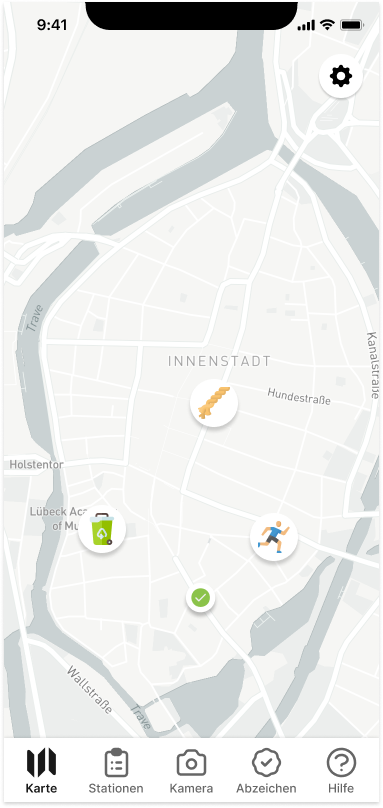
\includegraphics[width=.9\linewidth]{prototype/Karte.png}
    \end{minipage}%
    \begin{minipage}{.33\textwidth}
        \centering
        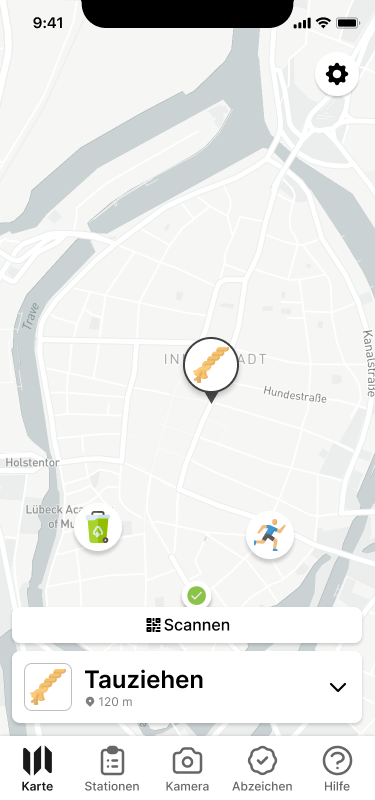
\includegraphics[width=.9\linewidth]{prototype/Karte-1.png}
    \end{minipage}
    \begin{minipage}{.33\textwidth}
        \centering
        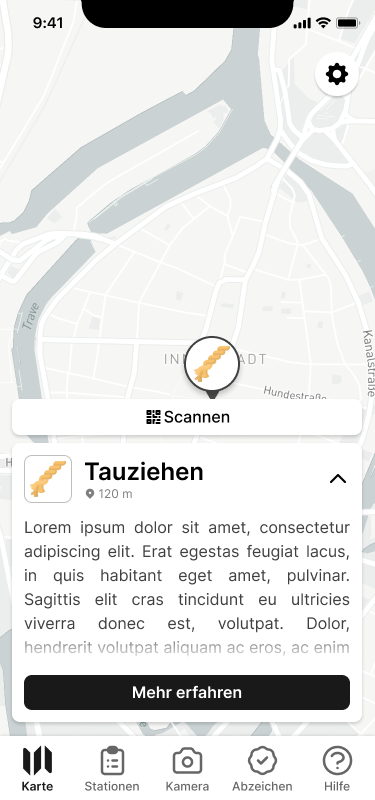
\includegraphics[width=.9\linewidth]{prototype/Karte-2.png}
    \end{minipage}
    \caption{Interaktive Karte mit Projektstandorten: nichts ausgewählt (links), ausgewählt (mittig), ausgewählt und aufgeklappt (rechts)}
    \label{fig:prototype-map}
\end{figure}

Aufgrund des variablen räumlichen Kontextes ist eine Verteilung der Stationen
über Kilometer große Räume möglich. Hierdurch ist die Distanz zu den
verschiedenen Stationen eine durchaus wichtige Information für Teilnehmende
(H2). Als Konsequenz wird die Distanz in verschiedenen relevanten Stellen des
User-Interfaces angezeigt. Eine dieser Stellen ist die interaktive Karte der
Stationen, insbesondere das Pop-up. Jenes wurde um die Distanz zur zugehörigen
Station ergänzt. Des Weiteren wird die Kurzbeschreibung standardmäßig
eingeklappt (s. \autoref{fig:prototype-map}, mittig), um Teilnehmende nicht mit
zu vielen Informationen zu konfrontieren (H7, H8). Zudem wird das Icon der
Station nun ebenfalls in das Pop-up eingebunden, da im Gegensatz zu den
generischen Planeten der EMI-Award-App, die Icons der Stationen von
Veranstaltenden selbst bestimmt werden. Somit werden die Icons der Stationen mit
diesen assoziiert, was die Wiedererkennung im Rest der Benutzeroberfläche
erleichtert (H6). Eine weitere Ergänzung stellt ein „Jetzt Scannen“-Button dar,
welcher direkt zur Kamera navigiert, um die Navigation zu dieser zu erleichtern
(H7) und gleichzeitig als \textit{In-Context}-Hilfe dient (H6). Um den Fokus auf
unbesuchte Stationen zu lenken, werden besuchte Stationen zudem mit einem Haken
als solche markiert und kleiner dargestellt (s. \autoref{fig:prototype-map},
links). Zusätzlich können besuchte Stationen auch komplett ausgeblendet werden.
Beide Maßnahmen zielen darauf ab, irrelevante Informationen auf der
Benutzeroberfläche zu vermindern oder zu vermeiden (H8). Hingegen wird die aktiv
ausgewählte Station durch eine Umrandung noch zusätzlich hervorgehoben.
Insgesamt wird die Struktur und Position des Pop-up angepasst, um sie populären
Apps mit ähnlichen Funktionen anzugleichen, da die Umgangsweise mit diesen
bereits bekannt ist und somit übertragen werden kann (H4).

\begin{figure}[htpb]
    \centering
    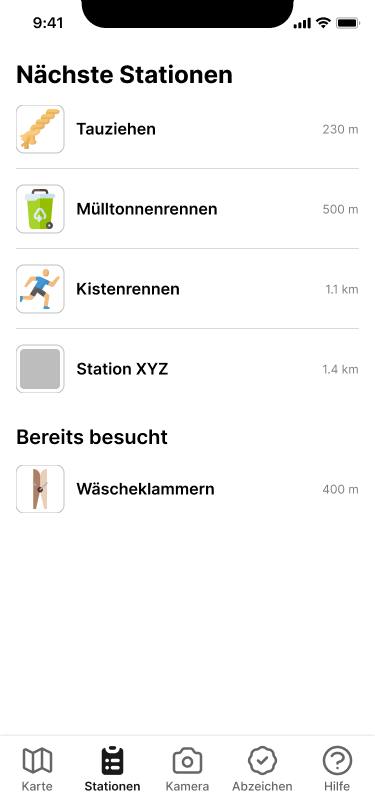
\includegraphics[width=.3\linewidth]{prototype/Stationen.png}
    \caption{Stationsauflistung}
    \label{fig:prototype-stations-list}
\end{figure}

Auch in der Stationsauflistung stellt die Distanz eine wichtige Information dar.
Somit wird für jeden Eintrag die Distanz angezeigt, wobei die Einträge
zusätzlich nach Distanz aufsteigend sortiert werden. Außerdem werden Stationen
nach „offen“ und „besucht“ gefiltert, wobei standardmäßig die Kategorie „offen“
angezeigt wird (s. \autoref{fig:prototype-stations-list}). Sowohl die Sortierung als auch die Filterung dienen dazu,
Teilnehmenden zuerst die relevantesten Informationen zu präsentieren (H8).
Konkret sind hiermit die nächstgelegenen unbesuchten Stationen gemeint. Des
Weiteren werden für die Einträge die jeweiligen Stationsicons verwendet. Diese
ersetzten die Bildvorschau der EMI-Award-App, da mediale Inhalte nicht mehr
zwingend benötigt werden, Icons hingegen schon.

\begin{figure}[htpb]
    \begin{minipage}{.5\textwidth}
        \centering
        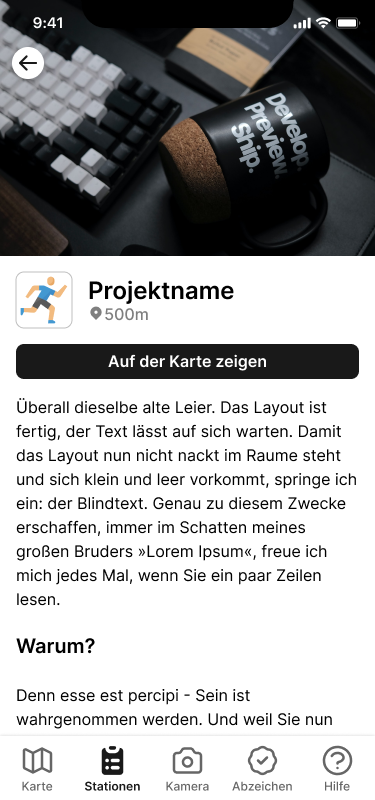
\includegraphics[width=.6\linewidth]{prototype/Stationen-1.png}
    \end{minipage}%
    \begin{minipage}{.5\textwidth}
        \centering
        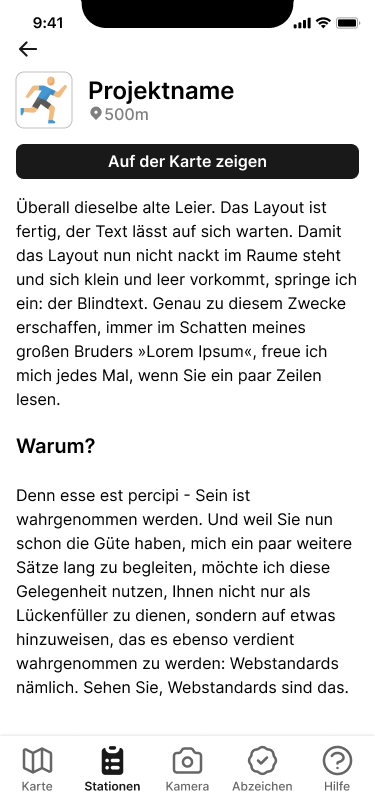
\includegraphics[width=.6\linewidth]{prototype/Stationen-2.png}
    \end{minipage}
    \caption{Stationsansicht: mit (links) und ohne (rechts) mediale Inhalte}
    \label{fig:prototype-stations-one}
\end{figure}

Die Stationsansicht wurde ebenfalls um die Distanz ergänzt und das
Wechseln zur Karte deutlich hervorgehoben. Da die Einbindung von medialen
Inhalten nicht zwingend erforderlich ist, wurde dies im Entwurf berücksichtigt
(vgl. \autoref{fig:prototype-stations-one}).

\begin{figure}[htpb]
    \begin{minipage}{.5\textwidth}
        \centering
        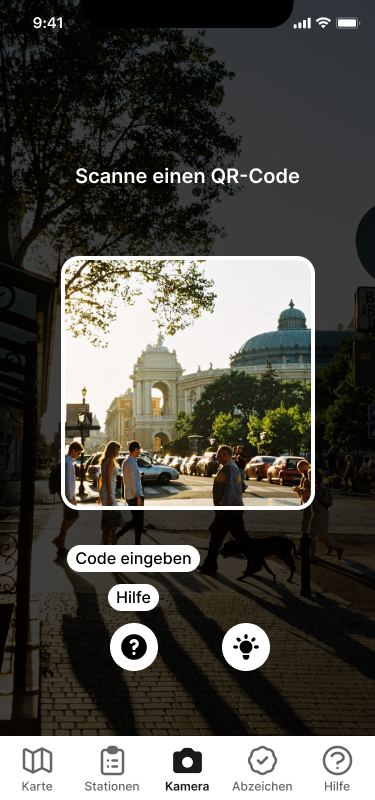
\includegraphics[width=.6\linewidth]{prototype/Kamera-1.png}
    \end{minipage}%
    \begin{minipage}{.5\textwidth}
        \centering
        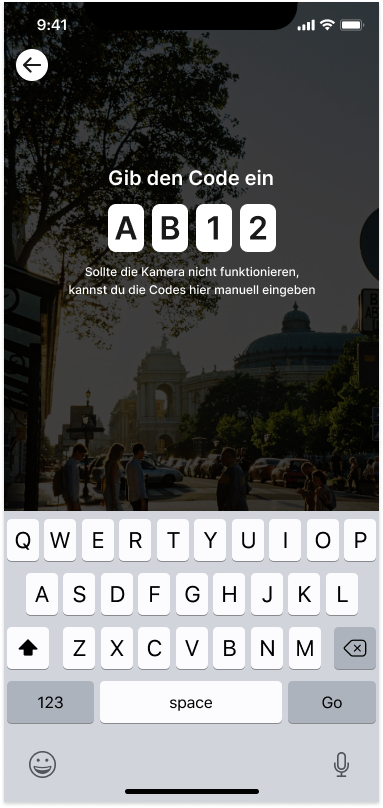
\includegraphics[width=.6\linewidth]{prototype/Kamera-2.png}
    \end{minipage}
    \caption{Kameraansicht: QR-Scanner (links) und manuelle Eingabe (rechts)}
    \label{fig:prototype-camera}
\end{figure}

Um die Scanner-Funktion der Kameraansicht ersichtlicher zu gestalten, wurde das
Design an gängige QR-Scanner angepasst (H4). Hierzu wurde der Scannerbereich mit
einem weißen Rand versehen und der restliche Bereich abgedunkelt (s.
\autoref{fig:prototype-camera}). Zudem wurden die Icons zur verbesserten
Sichtbarkeit zentraler positioniert und zusammengeführt. Die manuelle
Codeeingabe und Hilfe sind mit dem Antippen des Fragezeichen-Icons erreichbar,
während die Taschenlampe angezeigt wird, wenn das Gerät die Funktionalität
unterstützt. Da die Codeeingabe nur schwer durch ein eindeutiges Icon
darstellbar ist, wurde sich bewusst entschieden, die Funktionalität auszuschreiben.

\begin{figure}[htpb]
    \begin{minipage}{.5\textwidth}
        \centering
        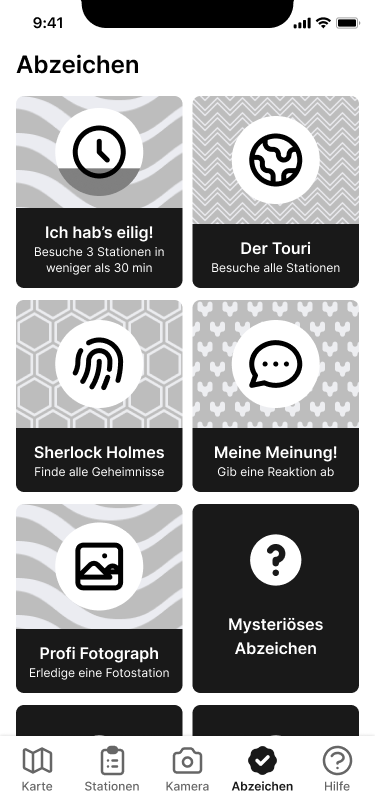
\includegraphics[width=.6\linewidth]{prototype/Abzeichen.png}
    \end{minipage}%
    \begin{minipage}{.5\textwidth}
        \centering
        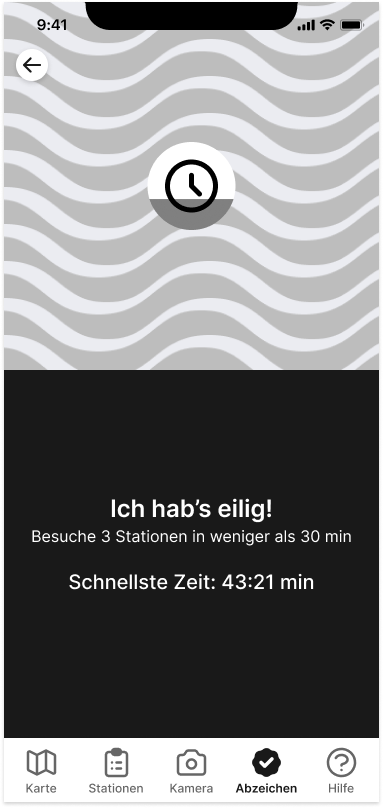
\includegraphics[width=.6\linewidth]{prototype/Abzeichen-1.png}
    \end{minipage}
    \caption{Abzeichen: Übersicht (links) und einzelne Ansicht (rechts)}
    \label{fig:prototype-achievement}
\end{figure}

Die einzelnen Abzeichen der Abzeichenansicht unterschieden sich in der
EMI-Award-App lediglich durch ihre Farbe. Um Veranstaltenden möglichst viele
Freiheiten in der Anpassung zu geben, kann für jedes Abzeichen ein Icon
festgelegt werden. Dies ersetzt die festen Icons der EMI-Award-App. Zusätzlich
wird jedes Abzeichen mit einem zufälligen Muster hinterlegt (s.
\autoref{fig:prototype-achievement}, links), um den Wiedererkennungswert und die
Differenzierbarkeit zu steigern. Außerdem erleichtert dies später die farbliche
Anpassung an die Veranstaltung (\anfref{F130}). Zudem wurde eine Einzelansicht
für Abzeichen hinzugefügt. Diese wird für die Text- und Bildabzeichen (Ft-T-8)
zum Einreichen benötigt und gibt Platz für ausführlichere Erklärungen oder
weiteren Informationen zu Abzeichen (s. \autoref{fig:prototype-achievement},
rechts).

\begin{figure}[htpb]
    \begin{minipage}{.5\textwidth}
        \centering
        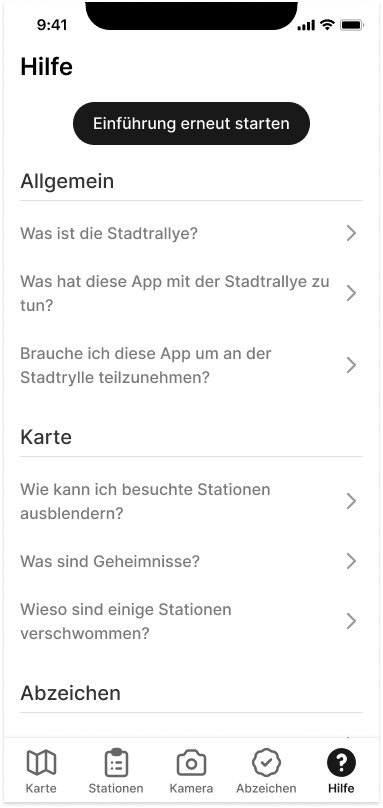
\includegraphics[width=.6\linewidth]{prototype/Hilfe.png}
    \end{minipage}%
    \begin{minipage}{.5\textwidth}
        \centering
        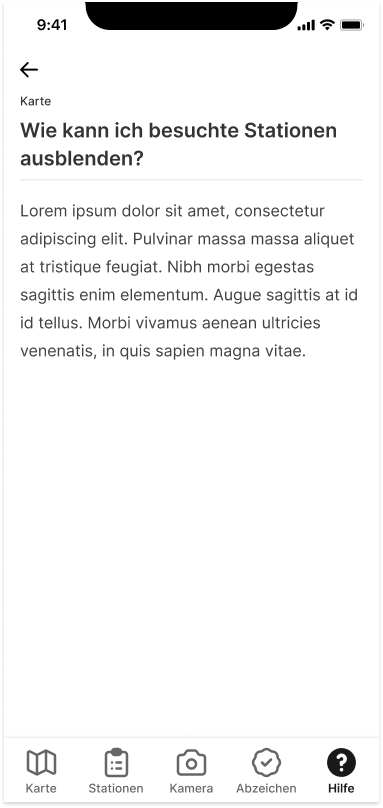
\includegraphics[width=.6\linewidth]{prototype/Hilfe-1.png}
    \end{minipage}
    \caption{Hilfe: Übersicht (links) und einzelne Ansicht (rechts)}
    \label{fig:prototype-help}
\end{figure}

Durch die in \autoref{sec:concept-func} beschriebenen Überarbeitung der
Hilfe-Funktion, muss die Benutzeroberfläche angepasst werden. Um die
Fragen übersichtlich anzuzeigen, werden sie nach den erstellten Kategorien
gruppiert präsentiert. Die Kategorien werden dabei durch die jeweilige
Überschrift abgegrenzt. Die Antwort zu den einzelnen Fragen wird wiederum in
einer Einzelansicht dargestellt. Zudem wird über einen Button im oberen Bereich
die Möglichkeit gegeben, die Einführung in die Veranstaltung (Ft-T-6) erneut zu durchlaufen.



% Design System
% - Schriftgrößen
% - Schriftgewichtungen
% - Farblos -> Anpassbar
%
% Schriftart: Inter
% - Hohes Mittellängen-Schriftgrößen Verhältnis -> Sehr gut lesbar (DVSG)
%
% Schriftgröße: Laut DVSG Rechner mindestens 13px bei 30cm, 0.5 Visus, 0.7 MSV
% und 150 ppi
%
% Iconsatz: Heroicons

% - Icons im Popup, da klein und durch Veranstalter bestimmbar statt generischer
%   Planet
% - Durch Distanz + Icon an Info dazu, sehr viele Informationen -> Ausblenden
%   von Sekundär Informationen (H8)

\section{Frameworks}

\section{Systemarchitektur}

% Speichern von Nutzerdaten ohne konkrete Anmeldung

% Usability von interaktiven Karten
% - Alter
% - Behinderung
% - Technikaffinität

% Usability QR-Code Reader



%!%%%%%%%%%%!%
%! Frontend !%
%!%%%%%%%%%%!%
% inclusive Design
%   - Mehrsprachig
%   - A11y (Aria, W3C Empfehlungen)

% Auf "Refactoring UI"-Standards geachtet

% Tailwindcss Design-System verwendet

%!%%%%%%%%%!%
%! Backend !%
%!%%%%%%%%%!%
% Komplexe Modellierung: Gruppen / Einzel

% Darstellung der Datenbank Relation

% Strukturierung der API
%   - Gruppen API
%   - Besuchs API
%   - Benachrichtigungs API
%   - Abzeichen API

\section{Implikation für Implementierung}

% Gedanken zur technischen Umsetzung der EMI-App
%   - Vor-/Nachteile Web/Native
%   - Library Entscheidungen